% Created 2023-11-11 Sat 18:00
% Intended LaTeX compiler: pdflatex
\documentclass[ee,msthesis]{usuthesis}
\usepackage[utf8]{inputenc}
\usepackage[T1]{fontenc}
\usepackage{graphicx}
\usepackage{longtable}
\usepackage{wrapfig}
\usepackage{rotating}
\usepackage[normalem]{ulem}
\usepackage{amsmath}
\usepackage{amssymb}
\usepackage{capt-of}
\usepackage{hyperref}
\usepackage{amsmath}                         % Miscellaneous enhancements for mathematics
\usepackage{amssymb}                         % Math symbols
\usepackage{algorithm2e}                    % Algorithms
\usepackage{amsfonts}                       % Cool math fonts
\usepackage{booktabs}                       % Used for lines in table
\usepackage{lipsum}                         % Dummy filler text
\usepackage{multicol}                       % Add capability to make columns
\usepackage{multirow}                       % Add capability to make rows
\usepackage{pgfgantt}                       % Add capability to create gantt charts
\usepackage{standalone}                     % Allow standalone documents
\usepackage{subcaption}                     % Allow subfigures
\usepackage{subfloat}                       % Subfigures
\usepackage{tabularx}                        % Add more contol to tables
\usepackage{listings}                       % Display code
\usepackage{doi}                            % Hyperling DOI
\usepackage{hyperref}                       % Cool clean hyperlinks
\usetikzlibrary{arrows.meta}                % Arrows for tikz
\renewcommand*{\chapterautorefname}{Chapter}
\renewcommand*{\sectionautorefname}{Section}
\renewcommand*{\subsectionautorefname}{Subsection}
\renewcommand*{\subsubsectionautorefname}{Subsubsection}
\renewcommand*{\paragraphautorefname}{Paragraph}
\renewcommand*{\algorithmautorefname}{Algorithm}
\newcommand{\definitionautorefname}{Definition}
\newcommand{\Or}{\textbf{ or }}
\renewcommand*{\And}{\textbf{ and }}
\newcommand\mycommfont[1]{\footnotesize\ttfamily\textcolor{gray}{#1}}
\newcommand{\T}{\mathcal{T}}                % To make it clear the difference
\newcommand{\Tau}{T}                        % between Tau and T
\newcommand{\AC}{AC(u, d, v, \eta)}            % Set the parameters for AC once
\newcommand{\PC}{PC(u, d, v)}               % Set the parameters for PC once
\newcommand{\ACi}{AC(u_i, d_i, v_i, \eta_i)}% Set the parameters for AC once
\newcommand{\PCi}{PC(u_i, d_i, v_i)}        % Set the parameters for PC once
\newcommand{\Not}{\textbf{not }}            % Custom `not' operator
\newcommand{\visit}{(b_i, a_i, e_i, u_i, d_i, v_i, \eta_i, \xi_i)}
\newcommand{\I}{\mathbb{I}}                 % Set of visit tuples
\newcommand{\C}{\mathbb{C}}                 % Charger availability information
\newcommand{\U}{\mathcal{U}}                % Uniform distribution
\newcommand{\Sol}{\mathbb{S}}               % A shorthand for visit tuple
\newcommand{\M}{\mathbb{M}}                 % A shorthand for the metadata
\newcommand{\Hd}{\mathbb{H}}                % Set of discrete times
\newcommand{\Nu}{\mathcal{V}}               % Draw a nice Nu
\newcommand{\Iset}{\mathcal{I}}             % Set of visits 1-I
\newcommand{\Isetinit}{\mathcal{I}_0}       % Set of visits inital visits
\newcommand{\Isetfinal}{\mathcal{I}_f}      % Set of visits final visits
\newcommand{\Bset}{\mathcal{B}}             % Set of visits 1-B
\newcommand{\Qset}{\mathcal{Q}}             % Set of visits 1-Q
\newcommand{\Jset}{\mathcal{J}}             % Set of visits 1-J
\newcommand{\Jsetq}{\mathbb{J}}             % Set of visits 1-J for queue active times
\newcommand{\Hset}{\mathcal{H}}             % Set of visits 1-H
% The Committee
\majorprof{Dr. Droge, Ph.D.}
\firstreader{Dr. Gunther, Ph.D.}
\secondreader{Dr. Sarsilmaz, Ph.D.}

% Graduate Dean
\graddean{ D. Richard Cutler, Ph.D.}
\deantitle{ Vice Provost of Graduate Studies}

% Degree Information
\degree{Master of Science}
\month{Dec}
\gradyear{2023}
\newtheorem{definition}{Definition}[section]
\author{Alexander Brown}
\date{}
\title{The Simulated Annealing Fully Fuzzy Position Allocation Problem Utilizing Mixed Integer Linear Programming Constraints with Non-Linear Battery Dynamics}
\hypersetup{
 pdfauthor={Alexander Brown},
 pdftitle={The Simulated Annealing Fully Fuzzy Position Allocation Problem Utilizing Mixed Integer Linear Programming Constraints with Non-Linear Battery Dynamics},
 pdfkeywords={},
 pdfsubject={},
 pdfcreator={Emacs 29.1 (Org mode 9.6.11)}, 
 pdflang={English}}
\begin{document}

\let\ref\autoref                            % Redifine `\ref` as `\autoref` because lazy
\SetCommentSty{mycommfont}                  % Set the comment color

\preliminaries   % set frontmatter style

\maketitle

\tableofcontents
\listoftables
\listoffigures

\body  % set main body style

\chapter{INTRODUCTION}
\label{sec:introduction}
Public transportation systems are crucial in any urban area; however, the increased awareness and concern of
environmental impacts of petroleum based public transportation has driven an effort to reduce the pollutant footprint
\cite{de-2014-simul-elect,xylia-2018-role-charg,guida-2017-zeeus-repor-europ,li-2016-batter-elect}. Particularly,
the electrification of public bus transportation via battery power, i.e., battery electric buses (BEBs), has received
significant attention \cite{li-2016-batter-elect}. Although the technology provides benefits beyond reduction in
emissions, such as lower driving costs, lower maintenance costs, and reduced vehicle noise, battery powered systems
introduce new challenges such as larger upfront costs, and potentially several hours long ``refueling'' periods
\cite{xylia-2018-role-charg,li-2016-batter-elect}. Furthermore, the problem is exacerbated by the constraints of the
transit schedule to which the fleet must adhere, the limited amount of chargers available, and the adverse affects in
the health of the battery due to fast charging \cite{lutsey-2019-updat-elect}.

BEBs have been in service for many major markets, North America, Europe, and China, for more than a decade with expected
growth in the near future \cite{deng-2021-survey-elect}. The Asia Pacific market is forecasted to dominate the sales
and some major companies of the industry have also begun to enter the global market such as Volvo, BYD, and Proterra by
2025 \cite{deng-2021-survey-elect}. Much focus has been placed on the engineering of individual BEBs such as battery
type, brake regenerative charging, optimal battery charging, and battery degradation \cite{chen-2008-desig-grey,abdollahi-2016-optim-batter,kuhne-2010-elect,deng-2021-survey-elect}. The interest of route scheduling, charging
fleets, and optimizing the infrastructure are problems of more recent interest and are therefore timely and increasingly
relevant problems as EV/BEBs become more commonplace \cite{hoke-2014-accoun-lithium,sebastiani-2016-evaluat-elect,wei-2018-optim-spatio}.

The literature shows an interest in solving the problem of assigning BEBs to charging queues or optimizing their
infrastructure \cite{wei-2018-optim-spatio,sebastiani-2016-evaluat-elect,hoke-2014-accoun-lithium,wang-2017-elect-vehic}. In fact, many works attempt to solve both problems simultanously
barring some simplification whether it be only allowing chargers of a single type
\cite{he-2020-optim-charg,tang-2019-robus-sched}. If multiple chargers are used, then one of each type is assigned at
each location. Others have also assumed that a BEB shall recieve full charge upon each arrival
\cite{wei-2018-optim-spatio,wang-2017-elect-vehic,zhou-2020-bi-objec,wang-2017-optim-rechar}. Some works on the
stochastic effects of energy consumption while on route for a BEB as well as trip times \cite{zhou-2020-collab-optim,bie-2021-optim-elect}. One other source, as far as the reseach for this work has shown, describes a method of producing
a BEB charge schedule wih a high fidelity while accounting for multiple charger times as well as being able to minimize
over the total charger count \cite{whitaker-2023-a-network}.

The work described in this proposal is similar to the work in \cite{whitaker-2023-a-network}; however provides an
alternate method of modeling the problem in what is known as the Position Allocation Problem (PAP). The PAP is modeled
after the Berth Allocation Problem (BAP), which was designed to optimally schedule cargo vessels to be berthed and
serviced \cite{buhrkal-2011-model-discr,imai-2001-dynam-berth,frojan-2015-contin-berth}. The PAP utilizes this
notion to develop a model of assigning EVs to queue in ordered to be charged \cite{qarebagh-2019-optim-sched}.

Because of the PAP's extremely close modeling methods to the BAP, literature from the BAP can (and will) provide support
for the development of the PAP in this work. The BAP has been studied in literature since the 1990s and provides a depth
of work to derive from \cite{rodrigues-2022-berth}. The proposed work also intends to introduce a sense of robustness
by allowing uncertainty in the arrival times of the BEBs. By ``fuzzifying'' the model, the ``fuzzy'' variables are allowed
to have upper and lower bounds for which the model can provide solutions for. The work to be introduced promises much
potential for further research and development in regard to scheduling BEBs. What follows is a proposal for a Simulated
Annealing (SA) implementation and extension of the PAP utilizing Fully Fuzzy Mixed Integer Linear Programming (FFMILP)
constraints with non-linear battery dynamics.

In the next section, a review of relevant literature of BEBs is introduced and discussed. Background and a problem
statement will be elaborated further to provide context and a required basis of understanding prior to discussing the
objectives and approaches in \ref{sec:objectives} and \ref{sec:approach}, respectively. The BEB queue scheduling problem discussed
throughout this section is of particular interest at this time in the BEB industry and requires more attention. The
research proposed directly approaches this problem by improving upon existing implementations to provide a robust and
accurate solution. In the subsequent sections the objectives will be introduced in \ref{sec:objectives} and the approach for
each objective will be discussed in \ref{sec:approach}.
\chapter{OBJECTIVES}
\label{sec:objectives}
The field of BEB research provides exciting many avenues and is continuing to gain traction in industry as BEBs replace
their gasoline counterparts. This work will introduce a novel approach to BEB scheduling that minimizes monetary costs
for the user, provides a robust solution, and includes an accurate dynamic battery model. The PAP provides a solid
foundation from which this work derived. However, the PAP does not perfectly encapsulate the problem and thus needs some
modifications to accommodate the BEB model. The PAP does not account for the revisits of a BEB and therefore the
State-Of-Charge (SOC) cannot be tracked. The model does not account for multiple charger types, and in fact models the
charger as a single continuous bar. These accommodations must be accounted for and are included in the objectives for
the proposed BEB charging plan below.

\begin{itemize}
\item \textbf{Objective 1}: Mathematically model the PAP to optimally assign BEBs to queues with unknown charging times to allow consideration of consumption cost and battery health

\begin{itemize}
\item \textbf{Task 1.1}: Modify PAP to enable multiple visits by a BEB with variable charger duration per visit.

\item \textbf{Task 1.2}: Incorporate heterogeneous charger capabilities into the PAP to model slow and fast charging, minimize
and total charger count. Slow charging will be incentivized for battery health and consumption cost.
\end{itemize}

\item \textbf{Objective 2}: Develop robust charger allocation capabilities to account for BEB arrival time uncertainties and non-linear battery dynamics

\begin{itemize}
\item \textbf{Task 2.1}: Incorporate non-linear battery dynamics into the FFLP PAP model

\item \textbf{Task 2.2}: Model the PAP as an FFLP to allow for uncertain BEB arrival/charge/departure times. An optimal solution shall be
produced, but with added flexibility to its application.
\end{itemize}
\end{itemize}
\chapter{BACKGROUND AND RELATED WORK}
\label{sec:background-and-related-work}
The BEB queue scheduling problem is one that has been of increasing interest and relevancy in the EV/BEB industry. It is
thus important to address the state of the art by introducing relevant problems in BEB queue scheduling, which will be
addressed first. A detailed problem description shall then be presented to give a better understanding of the
proposition moving forward, and then miscellaneous introductory theory will be presented that.

\section{State Of The Art of Battery Electric Bus Charging}
\label{sec:state-of-the-art}
Two of the main problems that have been of recent interest are solving the problems of route scheduling and charging
fleets as well as determining the infrastructure upon which they rely. In fact, the prospect of solving both problems
simultaneously has received much attention \cite{wei-2018-optim-spatio,sebastiani-2016-evaluat-elect,hoke-2014-accoun-lithium,wang-2017-elect-vehic}. These problems vary by including assignment of buses to routes
\cite{rinaldi-2020-mixed-fleet,zhou-2020-collab-optim,tang-2019-robus-sched,li-2014-trans-bus}, determining
whether a set of existing combustion based buses should be replaced with BEBs \cite{zhou-2020-bi-objec,duan-2021-refor-mixed,rinaldi-2020-mixed-fleet,zhou-2020-collab-optim}, and accounting for uncertainties
\cite{bie-2021-optim-elect,duan-2021-refor-mixed,tang-2019-robus-sched,ursavas-2016-optim-polic}. These problems
add additional complexities that warrant simplifications due to computational complexities.

Several simplifications are made throughout the literature to make these problems computationally feasible. These
simplifications to the charge scheduling model include utilizing only fast chargers while planning
\cite{wei-2018-optim-spatio,sebastiani-2016-evaluat-elect,wang-2017-optim-rechar,zhou-2020-bi-objec,yang-2018-charg-sched,wang-2017-elect-vehic,qin-2016-numer-analy,liu-2020-batter-elect}. If slow chargers are used,
they are only deployed at the one location with fast chargers being deployed elsewhere
\cite{he-2020-optim-charg,tang-2019-robus-sched}. Some approaches also simplify by assuming a full charge is always
achieved \cite{wei-2018-optim-spatio,wang-2017-elect-vehic,zhou-2020-bi-objec,wang-2017-optim-rechar}.

In some works, it was assumed that the charge received is proportional to the time spent on the charger
\cite{liu-2020-batter-elect,yang-2018-charg-sched}. While the linear battery dynamics is a valid assumption when the
battery SOC is below 80\% \cite{liu-2020-batter-elect}, non-linear battery dynamics can be implemented to more accurately
model the charge curve. A common way to model the non-linear battery dynamics is utilizing Constant Voltage (CV),
Constant Current (CC), and Constant Current Constant Voltage (CCCV) \cite{abdollahi-2016-optim-batter,chen-2008-desig-grey}. It has also been suggested that the dynamics can be modeled as a piecewise function containing a
linear and non-linear component from which a piecewise function approach may be taken for the CV and CC components
\cite{zhang-2021-optim-elect,abdollahi-2016-optim-batter}. Others have modeled the battery dynamics as a discrete
first order dynamics model \cite{whitaker-2023-a-network}. The first-order differential system, when provided a step
input, approximates the non-linear relationship between time and the current SOC \cite{whitaker-2023-a-network}.

Works concerning charge planning often use a version of the vehicle scheduling problem \cite{tang-2019-robus-sched,li-2014-trans-bus,he-2020-optim-charg}. Variants of this problem address infrastructure as well as determining
existing buses that should be replaced by a BEB \cite{zhou-2020-bi-objec,duan-2021-refor-mixed,rinaldi-2020-mixed-fleet,zhou-2020-collab-optim}. Other works introduce a directed graph approach to model the flow
of BEBs \cite{whitaker-2023-a-network,liu-2020-batter-elect}, where this concept was expanded to simultaneously
accounting for multiple charger types, partial charging, non-linear battery charge profiles
\cite{whitaker-2023-a-network}. The directed graph approach provides an easy method of modeling the scheduling by
discretizing the time horizon to \(n_Q\) sets of nodes. The nodes represent the chargers availability and can have a
maximum of one bus at a time. The buses can flow into a node to be charged and then later can exit allowing a new bus to
enter. Another method similar to the directed graph that fits the modeling of the BEB charging scenario is the PAP
\cite{qarebagh-2019-optim-sched}. The PAP is derived from the BAP which takes an input of vessel arrival times and
outputs the selection of the berthing quay. The PAP utilizes this model and redefines its inputs to EV arrival times and
outputs queues for the EVs to be charged. While the visits remain as discrete events, the time that the BEB is on the
charger is modeled in continuous time similar to \cite{frojan-2015-contin-berth,qarebagh-2019-optim-sched,zhou-2020-collab-optim}. Due to the close relationship between the BAP and PAP, BAP
literature may be used for the PAP. The literature shows methods of handling multiple quays (sets of chargers) to handle
general berthing scenarios \cite{frojan-2015-contin-berth,dai-2008-suppl-chain-analy}. Heuristic procedures for
quicker solve times have also been introduced \cite{imai-2001-dynam-berth}. Methods of defining static (full time
horizon) and dynamic (rolling-time horizon) models have been created for daily and real-time solutions, respectively,
and even fuzzy set theory has been applied to allow for more flexible schedules \cite{bello-2019-fuzzy-activ}.

An issue with the models introduced in the previous paragraph is the strict nature of the solutions produced. Fuzzy
mathematical programming is useful in situations where imprecise parameters exist \cite{bello-2019-fuzzy-activ}.
Previous work has utilized a stochastic approach to model uncertainties \cite{bie-2021-optim-elect,duan-2021-refor-mixed,tang-2019-robus-sched}. Work related to the BAP shows a Fully Fuzzy Linear Program (FFLP)
converts the FFLP to its ``crisp'' counterpart using one of various methods, a popular one being the Nasseri Method
\cite{bello-2019-fuzzy-activ}; however, to the extent of the research done for this work, FFLP has not been applied to
EV or BEB scheduling. FFLP provides a simple modeling solution that naturally describes the inaccuracies associated with
arrival times of BEBs. Furthermore, the result produced from an FFLP model describes a range of optimal solutions based
from the uncertainties defined by the input parameters.

\section{Mixed Integer Linear Programming}
\label{sec:orgdf96e46}

A mixed integer linear programming (MILP) problem is a class of constrained optimization in which one seeks to find a
set of continuous or integer values that maximizes or minimizes an objective function while satisfying a set of
constraints \cite{chen-2010-applied}. Given an objective function \(J\), decision variables (i.e. variables of
optimization) \(x_j \in \mathbb{R}\) and \(y_k \in \mathbb{Z}^+\), and input parameters \(c_j, d_k, a_{ij}, g_{ik}, b_i \in \mathbb{R}\), a MILP has a
mathematical structure represented as shown in \ref{eq:milp-structure} \cite{chen-2010-applied}

\begin{subequations}
\label{eq:milp-structure}
\begin{align}
&\text{max}        &J = \sum_j c_j x_j + \sum_k d_k y_k&         &               &\label{eq:fuzzy-milp-objective}\\
&\text{subject to} &\sum_j a_{ij} x_j + \sum_k g_{ik} y_k \le b_i&  &(i = 1,2,...,m)& \label{eq:fuzzy-milp-constraint}\\
&                  &x_j \ge 0&                              &(j = 1,2,...,n)& \label{eq:fuzzy-milp-continuous}\\
&                  &y_k \in \mathbb{Z^+}&                   &(k = 1,2,...,n)& \label{eq:fuzzy-milp-integer}\\
&\end{align}
\end{subequations}

The objective function in \ref{eq:fuzzy-milp-objective} comprises two parts, the continuous part, \(\sum_j c_j x_j\), and
integer part, \(\sum_k d_k y_k\). The decision variable of the first part, \(x_j\), is continuous whereas the decision variable
of the second, \(y_j\), is integer. Their respective input parameters may be integer or continuous, in the case of this
example they are modeled as continuous. The objective function's utility is to provide a numerical score to a system
(provided that a set of decision variables and input parameters are defined). While an individual score may not have any
intrinsic meaning, it provides a method of ranking different solutions of the same model. The constraint equations
(\ref{eq:fuzzy-milp-constraint} - \ref{eq:fuzzy-milp-integer}) must all be satisfied for the output of an objective
function to have any meaning. Thus, the constraint equations limit the solution space of the decision variables.
\ref{eq:fuzzy-milp-constraint} states that the summation of the products of the respective continuous and integer
decision variables and input parameters must be less than or equal to some value \(b_i\). \ref{eq:fuzzy-milp-continuous}
and \ref{eq:fuzzy-milp-integer} state that the decision variables \(x_j\) and \(y_k\), must be greater than or equal to 0,
respectively.

This formulation of the MILP in \ref{eq:milp-structure} is also referred to as ``crisp''. By this it is meant that each
variable in the formulation acts as an injective mapping to its number representation. In other words, every variable
has a one-to-one mapping from variable to value \cite{kaur-2016-introd-fuzzy}.

\section{Overview of the BAP}
\label{sec:overview-of-the-bap}
%% Rectangle packing figure
\begin{figure}
  \centering
  \includegraphics{sup-doc/milp-pap-paper-frontiers/img/spatiotemporal-packing}
  \caption{Example of rectangle packing problem. The large square represented by $O$ indicates the canstrained area that the set of shaded rectangles $\mathbb{O}$ must be placed within.}
  \label{fig:packexample}
\end{figure}

%% BAP/PAP solution plot example
\begin{figure}
  \centering
  \includegraphics{sup-doc/milp-pap-paper-frontiers/img/baprep}
  \caption{The representation of the berth-time space. The x and y-axis represent time and space, respectively. Along the y-axis, the dashed lines represent discrete berthing locations. These locations may be chosen to be continuous. The shaded rectangles represent scheduled vessels to be serviced. The height of each shaded rectangle represents the space taken on the berth and the width being the time to service said vessel. The vertical dashed lines are associated with vessel D and represent the arrival time, berthing time, serviced completion time, and departure time. Note that the arrival time may be before the berthing time and the completion time may before the departure time.}
  \label{fig:bap}
\end{figure}

The BAP is a rectangle packing problem where a set of rectangles, \(\mathbb{O}\), are attempted to be optimally placed in
a larger rectangle, \(O\), as shown in \autoref{fig:packexample}. The rectangle packing problem is an NP-hard problem that
can be used to describe many real life problems \cite{bruin-2013-rectan-packin,murata-1995-rectan}. In some of these
problems, the dimensions of \(\mathbb{O}\) are held constant such as in the problem of packing modules on a chip, where
the widths and height of the rectangles represent the physical width and heights of the modules
\cite{murata-1995-rectan}. Other problems, such as the BAP can allow one side of the rectangle to vary depending on its
assigned position (e.g. the varying lengths of the vessels) \cite{buhrkal-2011-model-discr}.

The BAP solves the problem of optimally assigning incoming vessels to berth positions to be serviced. The width and
 height of \(O\) time horizon \(T\) and represent the berth length \(S\), respectively. Similarly, the width and height for
 \(\mathbb{O}\) represent the time spent to service vessel \(i\) and the space taken by docking vessel \(i\), respectively. In
 the BAP, the vessel characteristics (length of the vessel, arrival time, handling time, desired departure time) are
 assumed to be known for all vessels to be serviced. A representation of a BAP solution is shown in \autoref{fig:bap}.
 The x and y-axis represent time and space, respectively. The grey squares, labeled A, B, C, and D, represent berthed
 vessels. The width of the boxes represent the time spent being serviced, and the height represents the amount of space
 the vessel requires on the berth. The vertical line adjacent ``Arrival Time'' represents the actual time that the
 vessel arrives and is available to be berthed. ``Berthing Time'' is the time the vessel is berthed and begins being
 serviced. ``Completion time'' represents the time at which the berthing space becomes available again.

\section{Overwiew of the PAP}
\label{sec:overview-of-the-pap}
The BAP defines the foundation of the PAP; however, there are some differences in the way the variables are interpreted. For
the \(i^{th}\) visit, starting service time is now the starting charge time, the berth location is now the charger queue
for assignment, and the service time is now the elapsed charge time. There are also a few clarifying concepts about how
the system is modeled. The PAP models the set of chargers as one continuous line; that is, the natural behavior of the
PAP model is to allow vehicles to be queued anywhere along the ``charge strip'' \([0,S]\). Similarly, the charge times are
continuous and can be placed anywhere on the time horizon, \([0,T]\), as long as the allocated times do not interfere with
other scheduled charge times.

\subsubsection{The PAP Formulation}
\label{sec:input-variables}
The BAP forms the basis of the PAP; however, there are some differences in the way the variables are interpreted. For
the \(i^{th}\) visit, starting service time, \(u_i\), is the starting charge time, the berth location, \(v_i\), is the charger
queue for assignment, and the service time, \(s_i\), is the elapsed charge time. There are also a few clarifying concepts
about how the system is modeled. The PAP models the set of chargers as one continuous line; that is, the natural
behavior of the PAP model is to allow vehicles to be queued anywhere along \([0,S]\). Similarly, the charge times are
continuous and can be placed anywhere on the time horizon, \([0,T]\), as long as the allocated times do not interfere with
other scheduled charge times. The PAP formulation's parameters can be divided into two categories: input parameters and
decision variables. Each type will now be introduced. The following parameters are constant inputs into the MILP.

\begin{itemize}
	\item $L$   : Size of the vehicle
	\item $T$   : time horizon
	\item $n_V$ : total number of incoming vehicles
	\item $s_i$ : charging time for vehicle $i;\; 1 \leq i \leq n_N$
	\item $l_i$ : width of vehicle $i;\; 1 \leq i \leq n_N$
	\item $a_i$ : arrival time of vehicle $i;\; 1 \leq i \leq n_N$
\end{itemize}

These constants define the problem bounds. The following list provides a series of decision variables used in the
formulation.

\begin{itemize}
    \item $u_i$    : starting charge time for vehicle $i;\; 1 \leq i \leq n_N$
    \item $v_i$    : assigned charge queue for vehicle $i;\; 1 \leq i \leq n_N$
    \item $d_i$    : departure time for vehicle $i;\; 1 \leq i \leq n_N$
    \item $\sigma_{ij}$ : binary variable that determines ordering of vehicles $i$ and $j$ in time
    \item $\psi_{ij}$ : binary variable that determines relative position of vehicles $i$ and $j$ when charging simultaneously
\end{itemize}

To determine the values for each of these decision variables, a MILP is formulated in \cite{qarebagh-2019-optim-sched}
and shown here for completeness.

\begin{equation}
	\label{eq:bapobjective}
	\min\; \sum_{i=1}^N (d_i - a_i)
\end{equation}

Subject to:
\begin{subequations}
\label{eq:bapconstrs}
\begin{align}
    u_j - u_i - s_i - (\sigma_{ij} - 1)T \geq 0                  \label{subeq:baptime}          \\
    v_j - v_i - l_i - (\psi_{ij} - 1)L \geq 0                \label{subeq:bapspace}           \\
    \sigma_{ij} + \sigma_{ji} + \psi_{ij} + \psi_{ji} \geq 1 \label{subeq:bapvalid_pos}     \\
    \sigma_{ij} + \sigma_{ji} \leq 1                              \label{subeq:bapsigma}        \\
    \psi_{ij} + \psi_{ji} \leq 1                              \label{subeq:bapdelta}        \\
    s_i + u_i = d_i                                               \label{subeq:bapdetach}       \\
    a_i \leq u_i \leq (T - s_i)                                   \label{subeq:bapvalid_starts} \\
    \sigma_{ij} \in \{0,1\},\;\psi_{ij} \in \{0,1\}\;           \label{subeq:bapsdspace}      \\
    v_i \in [0, L ]                                               \label{subeq:bapvspace}
\end{align}
\end{subequations}

\noindent

The objective function, \autoref{eq:bapobjective}, minimizes the time spent to service each vehicle by minimizing over
the sum of differences between the departure time, \(d_i\), and arrival time, \(a_i\). i.e., It seeks to get each vehicle
charged and on its way as quickly as possible.

\autoref{subeq:baptime}-\autoref{subeq:bapdelta} are used to ensure that individual rectangles do not overlap. For the
PAP, they ensure that two vehicles charging simultaneously are at different positions and, similarly, two vehicles that
have overlapping positions do not overlap temporally. \autoref{subeq:baptime} establishes temporal ordering when active
(\(\sigma_{ij}=1\)). Similarly, when \(\psi_{ij} =1\) in \autoref{subeq:bapspace} then spatial ordering is established. Constraints
\autoref{subeq:bapvalid_pos}-\autoref{subeq:bapdelta} enforce that spatial and/or temporal ordering is established
between each possible queue/vehicle pair. Constraints \autoref{subeq:bapsigma} and \autoref{subeq:bapdelta} enforce
consistency. For example, \autoref{subeq:bapsigma} enforces that vehicle \(i\) cannot come before vehicle \(j\) and vehicle
\(j\) simultaneously come before vehicle \(i\).

The last constraints force relationships between arrival time, charge start time, and departure time.
\autoref{subeq:bapdetach} states that the service start time, \(u_i\), plus the time to service vehicle \(i\), \(s_i\), must
equal the departure time, \(d_i\). \autoref{subeq:bapvalid_starts} enforces the arrival time, \(a_i\), to be less than or
equal to the service start time, \(u_i\), which in turn must be less than or equal to the latest time the vehicle may
begin to be serviced to stay within the time horizon. \autoref{subeq:bapsdspace} ensures that \(\sigma_{ij}\) and
\(\psi_{ij}\) are binary. \autoref{subeq:bapvspace} ensures that the assigned value of \(v_i\) is a valid charging position.
\begin{table}[!htpb]
  \caption{Notation used throughout the paper}
  \label{tab:variables}
  \centering
  \begin{tabularx}{\textwidth}{l l}
    \toprule
    \textbf{Variable} & \textbf{Description}                                                                               \\
    \toprule
    \multicolumn{2}{l}{Input values}                                                                                       \\
    $n_B$        & Number of buses                                                                                         \\
    $M$          & An arbitrary very large upper bound value                                                               \\
    $n_V$        & Number of total visits                                                                                  \\
    $n_Q$        & Number of queues                                                                                        \\
    $n_C$ 	 & Number of chargers                                                                                      \\
    $\mathbb{V}$ & Set of visit indices, $\mathbb{V} = \{1, ..., n_V\}$                                                    \\
    $\mathbb{B}$ & Set of bus indices, $\mathbb{B} = \{1, ..., n_B\}$                                                      \\
    $\mathbb{Q}$          & Set of queue indices, $\mathbb{Q} = \{1, ..., n_Q\}$                                                             \\
    $i,j$        & Indices used to refer to visits                                                                         \\
    $b$ 	 & Index used to refer to a bus                                                                            \\
    $q$ 	 & Index used to refer to a queue                                                                          \\
    \hline
    \multicolumn{2}{l}{Problem definition parameters}                                                                      \\
    $\Gamma$   & $\Gamma: \mathbb{V} \rightarrow \mathbb{B}$ with $\Gamma_i$ used to denote the bus for visit $i$                                   \\
    $\alpha_i$ & Initial charge percentage time for visit $i$                                                                   \\
    $\beta_i$ & Final charge percentage for bus $i$ at the end of the time horizon                                             \\
    $\epsilon_q$ & Cost of using charger $q$ per unit time                                                                        \\
    $\Upsilon$   & $\Upsilon: \mathbb{V} \rightarrow \mathbb{V}$ mapping a visit to the next visit by the same bus with $\Upsilon_i$ being the shorthand. \\
    $\kappa_b$ & Battery capacity for bus $b$                                                                                   \\
    $\Delta_i$ & Discharge of visit over route $i$                                                                              \\
    $\nu_b$ & Minimum charge allowed for bus $b$                                                                             \\
    $\tau_i$ & Time visit $i$ must depart the station                                                                         \\
    $\zeta_b$ & Discharge rate for bus $b$                                                                                     \\
    $a_i$ & Arrival time of visit  $i$                                                                                     \\
    $i_0$ & Indices associated with the initial arrival for every bus in $A$                                               \\
    $i_f$ & Indices associated with the final arrival for every bus in $A$                                                 \\
    $m_q$ & Cost of a visit being assigned to charger $q$                                                                  \\
    $r_q$ & Charge rate of charger $q$ per unit time                                                                       \\
    \hline
    \multicolumn{2}{l}{Decision Variables}                                                                                 \\
    $\psi_{ij}$ & Binary variable determining spatial ordering of vehicles $i$ and $j$                                       \\
    $\eta_i$    & Initial charge for visit $i$                                                                                \\
    $\sigma{ij}$ & Binary variable determining temporal ordering of vehicles $i$ and $j$                                       \\
    $d_i$    & Ending charge time for visit $i$                                                                            \\
    $g_{iq}$ & The charge gain for visit $i$ from charger $q$                                                              \\
    $s_i$    & Amount of time spent on charger for visit $i$                                                               \\
    $u_i$    & Starting charge time of visit $i$                                                                           \\
    $v_i$    & Assigned queue for visit $i$                                                                                \\
    $w_{iq}$ & Binary assignment variable for visit $i$ to queue $q$                                                       \\
    \bottomrule
  \end{tabularx}
\end{table}

\section{Fuzzy Preliminaries}
\label{sec:fuzzy-preliminaries}
This section introduces the concept of fuzzy set theory by providing some basic definitions. The theory is then built on
to discuss Fully Fuzzy Linear Programming (FFLP). FFLP is a branch of Linear Programming where some of the parameters
are allowed to have uncertainty which will be further elaborated on. In this section a method of constructing FFLP is
introduced. Once the FFLP model has been introduced, a derivation of the Fuzzy BAP (FBAP) is introduced and
discussed.

\subsection{Fuzzy Sets Theory}
\label{sec:fuzzy-sets-theory}
This section introduces the notion of fuzzy numbers and some basic definitions. Concepts from this section are
referenced from
\cite{zimmermann-2001-fuzzy-set,das-2016-mathem-model,yaghobi-2014-compar-fuzzy,bello-2019-fuzzy-activ,kaur-2016-introd-fuzzy}.

\subsubsection{Fuzzy Sets}
\label{sec:orge36b6a2}
A sensible method of introducing fuzzy sets is to begin by describing the familiar classic set. A classical (crisp) set
is defined as a collection of elements \(x \in X\). Crisp sets are binary, either an element belongs in the set, or it does
not \cite{zimmermann-2001-fuzzy-set}. For a fuzzy set, what is known as the characteristic function applies various
degrees of membership for elements of a given set \cite{zimmermann-2001-fuzzy-set}. The membership of a value in a
fuzzy set may vary may differ among other characteristic functions, but their intended purpose remains the same. The
membership function is said to be normalized if \(\text{sup}_x \mu_{\tilde{A}}(x) = 1\). As an example,
\ref{fig:lr-fuzzy-characteristic} demonstrates a membership function of an LR flat fuzzy number. For a formal definition, consider
the \ref{def:membership-function}:

\begin{subfigures}
    %%~~~~~~~~~~~~~~~~~~~~~~~~~~~~~~~~~~~~~~~~~~~~~~~~~~~~~~~~~~~~~~~~~~~~~~~~~~~~
    % LR Characteristic
    \begin{figure}[htpb]
    \centering
        \includestandalone{img/lr-flat-fuzzy}
        \caption{Example of a characteristic function for an LR flat fuzzy number. The line segments $[a,b)$ and $(c,d]$
          may be any function that satisfies \ref{def:reference-function}.}
        \label{fig:lr-fuzzy-characteristic}
    \end{figure}
    \hfill

    %%~~~~~~~~~~~~~~~~~~~~~~~~~~~~~~~~~~~~~~~~~~~~~~~~~~~~~~~~~~~~~~~~~~~~~~~~~~~~
    % Triangular characteristic
    \begin{figure}[htpb]
    \centering
        \includestandalone{img/trang-characteristic}
        \caption{Example plot of a characteristic function for a triangular fuzzy number.}
        \label{fig:triang-characteristic}
    \end{figure}
\end{subfigures}

\begin{definition}
\label{def:membership-function}
Let \(X\) be a collection of objects (often called the universe of discourse \cite{bello-2019-fuzzy-activ}). If \(X\) is denoted
generically by \(x\), then a fuzzy set \(\tilde{A}\) in \(X\) is a set of ordered pairs as shown in \ref{eq:membership-function}.

\begin{equation}
\label{eq:membership-function}
\tilde{A} = \{(x, \mu_{\tilde{A}}(x))| x\in X\}
\end{equation}

\noindent
\(\mu_{\tilde{A}}\) is called the membership function where \(\mu_{\tilde{A}}\) is the mapping \(\mu_{\tilde{A}} : X \rightarrow
[0,1]\); which assigns a real number to the interval \([0,1]\). The value of \(\mu_{\tilde{A}}\) represents the degree of
membership of \(x\) in \(\tilde{A}\).
\end{definition}

The shape of a fuzzy number type is defined by membership function. The general definition of fuzzy numbers is known as
LR fuzzy numbers \cite{kaur-2016-introd-fuzzy,zimmermann-2001-fuzzy-set}. \ref{def:reference-function} describes the
property that an \(L\) and \(R\) functions must have. The \(L\) function describes the properties that the left portion of the
fuzzy number has, and the \(R\) function describes the properties of the right.

\begin{definition}
\label{def:reference-function}
A function \(L:[0,\infty) \rightarrow [0,1]\) (or \(R:[0,\infty) \rightarrow [0,1]\)) is said to be reference a function of the fuzzy number if and only
if

\begin{enumerate}
\item \(L(0) = 1\) (or \(R(0) = 1\))
\item \(L\) (or \(R\)) is non-increasing on \([0,\infty)\)
\end{enumerate}
\end{definition}

The definition of an LR fuzzy number may now be developed given the basis of what properties an \(L\) (or \(R\)) function
must have. Consider \ref{def:lr-flat}-\ref{def:lr-non-negative}.

\begin{definition}
\label{def:lr-flat} A fuzzy number \(\tilde{A}\) defined on the set of real numbers, \(\mathbb{R}\), denoted as the tuple
\((m,n,\alpha,\beta)_{LR}\), is said to be an \(LR\) flat fuzzy number if its membership function \(\mu_{\tilde{A}}(x)\) is defined as
shown in \ref{eq:lr-flat-fuzzy}. Note that the underscore in the tuple, \((\cdot)_{LR}\) is used to indicate that the tuple is for
an LR fuzzy number.

\begin{equation}
\label{eq:lr-flat-fuzzy}
\mu_{\tilde{A}}(x) =
\begin{cases}
L(\frac{m-x}{\alpha}) & x \le m, \alpha > 0 \\
R(\frac{m-n}{\beta}) & x \ge m, \beta > 0 \\
1                & m \le x \le n
\end{cases}
\end{equation}
\end{definition}

\begin{definition}
\label{def:lr-non-negative}
An \(LR\) flat fuzzy number \(\tilde{A} = (m,n,\alpha,\beta)_{LR}\) is said to be a non-negative \(LR\) flat fuzzy number if and only
if \(m-\alpha \ge 0\) and is said to be non-positive \(LR\) flat fuzzy number if and only if \(m - \alpha \le 0\) is a real number.
\end{definition}

A simplification to the LR flat fuzzy number is the triangular fuzzy number, which is what will be utilized in this work
(\ref{fig:triang-characteristic}). The triangular fuzzy numbers shall also be defined over the set of real numbers \(\mathbb{R}\). Consider
\ref{def:triangular-fuzzy-number} - \ref{def:triangular-nonnegative}

\begin{definition}
\label{def:triangular-fuzzy-number} A fuzzy number that is represented by \(\tilde{A} = (a,b,c)\) is said to be triangular
if its membership function is defined as \ref{eq:triangular-fuzzy-number}. \ref{fig:triang-characteristic} depicts a visual
representation of a triangular fuzzy number.

\begin{equation}
\label{eq:triangular-fuzzy-number}
  \mu_{\tilde{A}}(x) =
  \begin{cases}
    \frac{(x-a)}{(b-a)} & a \le x \le b \\
    \frac{(c-x)}{(c-b)} & c \le x \le d \\
    0                   & \text{otherwise}
  \end{cases}
\end{equation}
\end{definition}

\begin{definition}
A fuzzy set \(\tilde{A}\) in \(\mathbb{R}\) is convex if and only if the membership function of \(\tilde{A}\) satisfies the inequality

\begin{equation*}
\mu_{\tilde{A}}[\beta x_1 + (1-\beta)x_2] \ge \text{min}[\mu_{\tilde{A}}(x_1), \mu_{\tilde{A}}(x_2)]\; \forall x_1, x_2 \in \mathbb{R}\; \beta \in [0,1]
\end{equation*}
\end{definition}

\begin{definition}
A fuzzy number is a normal and convex fuzzy set in \(\mathbb{R}\).
\end{definition}

\begin{definition}
\label{def:triangular-nonnegative}
The triangular fuzzy number \(\tilde{A}\) is nonnegative \(\iff\; a \ge 0\).
\end{definition}

\subsubsection{Fuzzy Arithmetic}
\label{sec:orga7bcc4b}
If two triangular fuzzy numbers \(\tilde{a}_1 = (a_1, a_2, a_3)\) and \(\tilde{b}_1 = (b_1, b_2, b_3)\) are nonnegative
then the following operations are defined in \ref{eq:fuzzy-arithmetic}.

\begin{equation}
\label{eq:fuzzy-arithmetic}
\begin{array}{lcl}
\tilde{a} \oplus \tilde{b} & = & (a_1 + b_1, a_2 + b_2, a_3 + b_3) \\
\tilde{a} \ominus \tilde{b} & = & (a_1 + b_3, a_2 + b_2, a_3 + b_1) \\
\tilde{a} \otimes \tilde{b} & = & (a_1 b_1, a_2 b_2, a_3 b_3)       \\
\end{array}
\end{equation}

\subsubsection{Comparing Fuzzy Numbers}
\label{sec:org629ad11}
Fuzzy numbers do not directly provide a method of ordering nor do they always provide an ordered set like real numbers
\cite{bello-2019-fuzzy-activ}. There are multiple methods for ordering fuzzy numbers, each coming with advantages and
disadvantages \cite{mccahon-1990-compar}. Different properties have been applied to justify comparison of fuzzy
numbers, such as: preference, rationality, and robustness
\cite{jimenez-2007-linear-progr,bello-2019-fuzzy-activ,kaur-2016-introd-fuzzy}. These methods are commonly known as
ranking functions or ordering functions \cite{bello-2019-fuzzy-activ,das-2016-mathem-model,kaur-2016-introd-fuzzy}.
Commonly, including in this work, the First index of Yager \cite{yager-1981-proced-order} is used. Let a fuzzy number
be represented as \(\tilde{A} = (a_1,a_2,...)\), then the First index of Yager is defined as \ref{eq:first-index-yager}.

\begin{equation}
\label{eq:first-index-yager}
\mathfrak{R}(\tilde{A}) = \frac{\sum_i a_i}{|\tilde{A}|}
\end{equation}

\noindent where \(|\cdot|\) represents the cardinality of the fuzzy number. In words, \ref{eq:first-index-yager} is merely the
average of the values in the fuzzy number. As a result, \(A \le B\) when \(\mathfrak{R}(\tilde{A}) \le \mathfrak{R}(\tilde{B})\)
\cite{bello-2019-fuzzy-activ}.

\subsection{Fully Fuzzy Linear Programming}
\label{sec:fully-fuzzy-linear-programming}
Much like the Linear Programs (LP), Fully Fuzzy Linear Programs (FFLP), it is a class of constrained optimization in
which one seeks to find a set of continuous variables that either maximizes or minimizes an objective function, \(J\),
while satisfying a set of constraints. The key difference in FFLP is that it is designed to accommodate imprecise
information \cite{bello-2019-fuzzy-activ,kaur-2016-introd-fuzzy}. In FFLP, the parameters and decision variables are
fuzzy and linear. A general FFLP is represented as shown in \ref{eq:general-fflp}. The subscripts \(\cdot_e\), \(\cdot_l\), and \(\cdot_g\)
indicate to equality, less than, and greater than constraints, respectively. As an example, the notation
\(\tilde{a}_{ej}\) is read as the \(e^{\text{th}}\) equality constraint for the \(j^{\text{th}}\) value in the fuzzy number
tuple for the fuzzy number \(\tilde{a}\). All variables besides \(\tilde{X} = (x_1, x_2, ...)\) are input variables.

\begin{equation}
\label{eq:general-fflp}
\begin{array}{lll}
\underset{{\tilde{x}}}{\text{max}} & J = \sum_j \tilde{C}_j \otimes \tilde{X}_j              &                 \\
\text{subject to}                  & \sum_j \tilde{a}_{ej} \otimes \tilde{x}_j = \tilde{b}_e &  \forall e = 1,2,3,... \\
                                   & \sum_j \tilde{a}_{lj} \otimes \tilde{x}_j \le \tilde{b}_l &  \forall l = 1,2,3,... \\
                                   & \sum_j \tilde{a}_{gj} \otimes \tilde{x}_j \ge \tilde{b}_l &  \forall g = 1,2,3,...
\end{array}
\end{equation}

There are many methods of solving FFLP
\cite{bello-2019-fuzzy-activ,kaur-2016-introd-fuzzy,ebrahimnejad-2016-new-method,nasseri-2013-fully}; however, a
common strategy is to convert the fuzzy model into a crisp model that can be solved using traditional methods
\cite{bello-2019-fuzzy-activ}. In \cite{nasseri-2013-fully,bello-2019-fuzzy-activ}, the method of converting the FFLP
into a crisp MILP is simply done by applying the ranking function to the objective function and breaking the constraints
down into a set of crisp constraints as shown in \ref{eq:nasseri-solution}. The constraints are separated according to the
definition of fuzzy set multiplication defined in \ref{eq:fuzzy-arithmetic}. The fuzzy number index is represented is the
exponent rather than the subscript to clearly distinguish between the indexed value in the fuzzy number and the
constraint index (i.e. \(\tilde{A} = (a^1,a^2,a^3)\)). Furthermore, it is assumed that the fuzzy numbers are nonnegative.
Although the following equation can be written in terms of general nonnegative LR fuzzy numbers, the parameters and
decision variables are written in terms of nonnegative triangular fuzzy numbers. Consider the equality constraint in
\ref{eq:general-fflp}. For each equality constraint there will be a lower, middle, and upper bound to the constraint. That
constitutes three equality constraints. \ref{eq:nasseri-solution} expands each constraint.

\begin{equation}
\label{eq:nasseri-solution}
\begin{array}{lclc}
\underset{{\tilde{x}}}{\text{max}}   & J = \mathfrak{R}\Big(\sum_j (c_j^1,c_j^2,c_j^3)(x_j^1,x_j^2,x_j^3)\Big) &\\
\text{subject to} & \sum_j a_{ej}^1 x_j^1 = b_e^1 & & \forall e = 1,2,3,... \\
                  & \sum_j a_{lj}^1 x_j^1 \le b_l^1 & & \forall l = 1,2,3,... \\
                  & \sum_j a_{gj}^1 x_j^1 \ge b_g^1  & & \forall g = 1,2,3,... \\
                  & \sum_j a_{ej}^2 x_j^2 = b_e^2 & & \forall e = 1,2,3,... \\
                  & \sum_j a_{lj}^2 x_j^2 \le b_l^2 & & \forall l = 1,2,3,... \\
                  & \sum_j a_{gj}^2 x_j^2 \ge b_g^2  & & \forall g = 1,2,3,... \\
                  & \sum_j a_{ej}^3 x_j^3 = b_e^3 & & \forall e = 1,2,3,... \\
                  & \sum_j a_{lj}^3 x_j^3 \le b_l^3 & & \forall l = 1,2,3,... \\
                  & \sum_j a_{gj}^3 x_j^3 \ge b_g^3  & & \forall g = 1,2,3,... \\
                  & x_j^2 - x_j^1 \ge 0         & x_j^3 - x_j^2 \ge 0 & \\
\end{array}
\end{equation}

\noindent Note the last constraint is defined to ensure the ordering of the triangular fuzzy number, \(x_j^1 \le x_j^2 \le x_j^3\).
To be more succinct, the FFLP can also equivalently be written as \ref{eq:nasseri-solution-condensed}.

\begin{equation}
\label{eq:nasseri-solution-condensed}
\begin{array}{llc}
\underset{{\tilde{x}}}{\text{max}} & J = \mathfrak{R}\Big(\sum_j (c_j^1,c_j^2,c_j^3) \otimes (x_j^1,x_j^2,x_j^3)\Big) &\\
\text{subject to} & \sum_j a_{ej}^k x_j^k = b_e^k &  \forall e = 1,2,3,... \\
                  & \sum_j a_{lj}^k x_j^k \le b_l^k &  \forall l = 1,2,3,... \\
                  & \sum_j a_{gj}^k x_j^k \ge b_g^k  &  \forall g = 1,2,3,... \\
                  & x_j^2 - x_j^1 \ge 0         & x_j^3 - x_j^2 \ge 0 \\
                  & \forall k \in \{1,2,...\}        &                  \\
\end{array}
\end{equation}

Where \(k\) has a max value equal to the cardinality to the type of fuzzy number being utilized. This can be further be
elaborated on by rewriting the inequality constraints as equality constraints by introducing slack variables. This is
useful as it represents the formulation in a standard form \cite{chen-2010-applied,vanderbei-2020-linear-progr}.

The given method is called the Kumar and Kaurs method \cite{kaur-2016-introd-fuzzy} which is similar in presentation of
the Nassiri method presented in \cite{bello-2019-fuzzy-activ}. Generally speaking, it is designed to solve FFLP
problems with inequality constraints having LR flat fuzzy numbers. Given the FFLP \ref{eq:general-fflp} and assuming that
\(\tilde{x}_j\) is an LR flat fuzzy number, the problem can be reformulated as \ref{eq:kumar-kaurs-fuzzy}
\cite{kaur-2016-introd-fuzzy}.

\begin{equation}
\label{eq:kumar-kaurs-fuzzy}
\begin{array}{lll}
\underset{{\tilde{x}}}{\text{max}} & J = \sum_j \tilde{C}_j \otimes \tilde{X}_j              &                                              \\
\text{subject to} & \sum_j \tilde{a}_{ej} \otimes \tilde{x}_j               = \tilde{b}_e & \forall e = 1,2,3,...                \\
                  & \sum_j \tilde{a}_{lj} \otimes \tilde{x}_j \oplus \tilde{S}_l = \tilde{b}_l \oplus \tilde{S'}_l & \forall l = 1,2,3,... \\
                  & \sum_j \tilde{a}_{gj} \otimes \tilde{x}_j \oplus \tilde{S}_g = \tilde{b}_g \oplus \tilde{S'}_g & \forall g = 1,2,3,... \\
                  & \mathfrak{R}(\tilde{S_l}) - \mathfrak{R}(\tilde{S_l'}) \ge 0                                     & \forall l = 1,2,3,...      \\
                  & \mathfrak{R}(\tilde{S_g}) - \mathfrak{R}(\tilde{S_g'}) \le 0                                     & \forall g = 1,2,3,...
\end{array}
\end{equation}

Expanding the set of equations and using the condensed notation in \ref{eq:nasseri-solution-condensed} we find
\ref{eq:kumar-kaurs-crisp} \cite{kaur-2016-introd-fuzzy}.

\begin{equation}
\label{eq:kumar-kaurs-crisp}
\begin{array}{lllc}
\underset{{\tilde{x}}}{\text{max}} & J = \mathfrak{R}\Big(\sum_j (c_j^1,c_j^2,c_j^3) \otimes (x_j^1,x_j^2,x_j^3)\Big) &                             &                                          \\
\text{subject to}  & \sum_j a_{ej}^k x_j^k = b_e^k                                &                                &   \forall e = 1,2,3,...        \\
                   & \sum_j a_{lj}^k x_j^k + s_l^k = s_l^{'k} + b_l^k                 &                                &   \forall l = 1,2,3,...       \\
                   & \sum_j a_{gj}^k x_j^k + s_g^k = s_l^{'k} + b_l^k                 &                                &   \forall g = 1,2,3,...      \\
                   & \mathfrak{R}(\tilde{S_l}) - \mathfrak{R}(\tilde{S_l'}) \ge 0                      &                                &  \forall l = 1,2,3,...          \\
                   & \mathfrak{R}(\tilde{S_g}) - \mathfrak{R}(\tilde{S_g'}) \le 0                      &                                &  \forall g = 1,2,3,...          \\
                   & x_j^2 - x_j^1 \ge 0                                         & x_j^3 - x_j^2 \ge 0              &         \\
                   & \forall k \in \{1,2,...\}                                            &                            &                       \\
\end{array}
\end{equation}

\subsubsection{Example}
\label{sec:fully-fuzzy-linear-programming-example}
To demonstrate the process of decomposing an FFLP into its crisp counterpart, a simple example is to be provided.
Consider the following convex non-negative triangular fuzzy FFLP show in \ref{eq:fflp-example}. The example is pulled from
\cite{nasseri-2013-fully}.

\begin{equation}
\label{eq:fflp-example}
\begin{array}{ll}
\underset{{\tilde{x}}}{\text{max}} & (1,2,3) \otimes \tilde{x}_1 \oplus (2,3,4) \otimes \tilde{x}_2 \\
\text{subject to}                  & (0,1,2) \otimes \tilde{x}_1 \oplus (1,2,3) \otimes \tilde{x}_2 \le (1,10,27) \\
                                   & (1,2,3) \otimes \tilde{x}_1 \oplus (0,1,2) \otimes \tilde{x}_2 \le (2,11,28)
\end{array}
\end{equation}

Using the method described in \ref{sec:fully-fuzzy-linear-programming}, the FFLP can be expanded into the following form
described in \ref{eq:fflp-example-crisp}. The objective function is expanded using the First Index of Yager. Each constraint
is then decomposed into three constraints with slack variables appended to the left-hand side and right-hand side of
their respective equation. The constraints for the slack variables are then included to ensure values of the triangular
fuzzy numbers for the slack variables are valid. \ref{eq:fflp-example-crisp} is now said to be a crisp representation of
\ref{eq:fflp-example} in standard form. Solving the FFLP utilizing the Octave LP module (using both the Nasseri and Kumar
methods to verify the results), the example problem has a solution as displayed in \ref{tab:fflp-example-solution}.

\begin{equation}
\label{eq:fflp-example-crisp}
\begin{array}{ll}
\underset{x}{\text{max}} & J = (\frac{1+2+3}{3})  (\frac{x_1^1 + x_1^2 + x_1^3}{3}) + (\frac{2,3,4}{3})  (\frac{x_2^1 + x_2^2 + x_2^3}{3}) \\
\text{subject to}        &  0x_1^1 + 1x_2^1 + s_1^1 = 1 + s_1^{1'}                                                                  \\
                         &  1x_1^2 + 2x_2^2 + s_1^2 = 10 + s_1^{2'}                                                                  \\
                         &  2x_1^3 + 3x_2^3 + s_1^3 = 27 + s_1^{3'}                                                                  \\
                         &  1x_1^1 + 0x_2^1 + s_1^1 = 2 + s_1^{1'}                                                                  \\
                         &  2x_1^2 + 1x_2^2 + s_1^2 = 11 + s_1^{2'}                                                                  \\
                         &  3x_1^3 + 2x_2^3 + s_1^3 = 28 + s_1^{3'}                                                                  \\
                         & \mathfrak{R}(\tilde{S_1}) - \mathfrak{R}(\tilde{S_1'}) \ge 0                                                                    \\
                         & \mathfrak{R}(\tilde{S_2}) - \mathfrak{R}(\tilde{S_2'}) \ge 0                                                                    \\
                         & x_j^2 - x_j^1 \ge 0                                                                                        \\
                         & x_j^3 - x_j^2 \ge 0                                                                                        \\
\end{array}
\end{equation}

\begin{table}[htbp]
\caption{\label{tab:fflp-example-solution}Solution to the crisp representation of the FFLP.}
\centering
\begin{tabular}{rrrrrrrrrrrr}
\(x_1^1\) & \(x_1^2\) & \(x_1^3\) & \(x_2^1\) & \(x_2^2\) & \(x_2^3\) & \(s_1^1\) & \(s_1^2\) & \(s_1^3\) & \(s_1^{1'}\) & \(s_1^{2'}\) & \(s_1^{3'}\)\\[0pt]
2 & 4 & 6 & 1 & 3 & 5 & 0 & 0 & 0 & 0 & 0 & 0\\[0pt]
\end{tabular}
\end{table}

\subsection{The Fuzzy BAP}
\label{sec:the-fuzzy-bap}
The following is a FFLP model to the continuous dynamical BAP that is able to allocate a quay to an incoming vessel
\cite{bello-2019-fuzzy-activ}. The model assumes that the arrival time, \(\tilde{a}\), berthing time, \(\tilde{u}\), and
handling time, \(\tilde{s}\), are assumed to be known, but imprecise. The objective of the model is to allocate all the
vessels to different quays, according to several constraints minimizing the total waiting time for all the vessels. The
model in its entirety is presented in \ref{eq:fuzzy-bap}. Note that a few modifications are made to the notation to
accommodate the notation of \cite{bello-2019-fuzzy-activ} while attempting to remain as consistent as possible with the
notation presented in this paper. In this section, \(Q\) refers to the set of quays. Furthermore, the model is defined
over multiple quays, thus indexing for position shall be written as \(v_{iq}\). Similarly, because of the added degree of
freedom, the spatiotemporal binary decision variables are represented as \(\sigma^q_{ij}\) and \(\psi^q_{ij}\). The \(\cdot^q\) term
represents the quay of interest.

\begin{equation}
\label{eq:fuzzy-bap}
\begin{array}{lll}
                   & \text{min} \sum_{q \in Q}\sum_{i \in I} (\tilde{u}_{iq} - \tilde{a}_i)           &                                \\
\text{Subject to:} &                                                             &                                    \\
                   & \sum_{q \in Q} v_{iq} = 1                                          & \forall i \in I;\; \forall q \in Q               \\
                   & \tilde{u}_{iq} \ge \tilde{a}_i                                 & \forall i \in I;\; \forall q \in Q                \\
                   & v_{iq} + l_i \le L_q                                           & \forall i \in I;\; \forall q \in Q                \\
                   & v_{iq} + l_i \le v_{jq} + M(1-\sigma^q_{ij})                           & \forall i,j \in I;\; i \ne j;\; \forall q \in Q   \\
                   & \tilde{u}_{iq} + \tilde{s}_i \le T                             & \forall i \in I;\; \forall q \in Q                \\
                   & \tilde{u}_{iq} + \tilde{s}_i \le \tilde{u}_{iq} + M(1-\psi^q_{ij})   & \forall i,j \in I;\; i \ne j;\; \forall q \in Q \\
\end{array}
\end{equation}

One may note the similarities to the previously presented BAB and PAP models in \ref{eq:fuzzy-bap}. It has yet been defined
in a way useful for the purposes for this work. The adaptation of the Fuzzy BAP (FBAP) to the Fuzzy PAP (FPAP) is
discussed next in \ref{sec:the-fuzzy-pap}. An example solution of \ref{eq:fuzzy-bap} for 2 quays, provided by
\cite{bello-2019-fuzzy-activ}, is shown in \ref{fig:bap-example-solution}. The figure represents the robustness of the fuzzy
berthing plan.

The lines below the small triangle represent the possible early berthing time. Similarly, the lines above the triangle
represent the possible late berthing of the vessel. The point where the small point resides is the optimum berthing
time. In \ref{fig:bap-example-solution} it appears that there are conflicts between some of the departures and arrivals of the
vessels due to the overlapping lines (e.g. V8 and V2). These overlapping arrivals and departures merely represent the
relationship of the fuzzy departure/arrival times of the vessels. For example, if V8 were to depart late, V2 has slack
to allow a late berthing and servicing. On the graph, that would represent a berthing time located somewhere above the
small triangle.

\begin{figure}[ht]
\centering
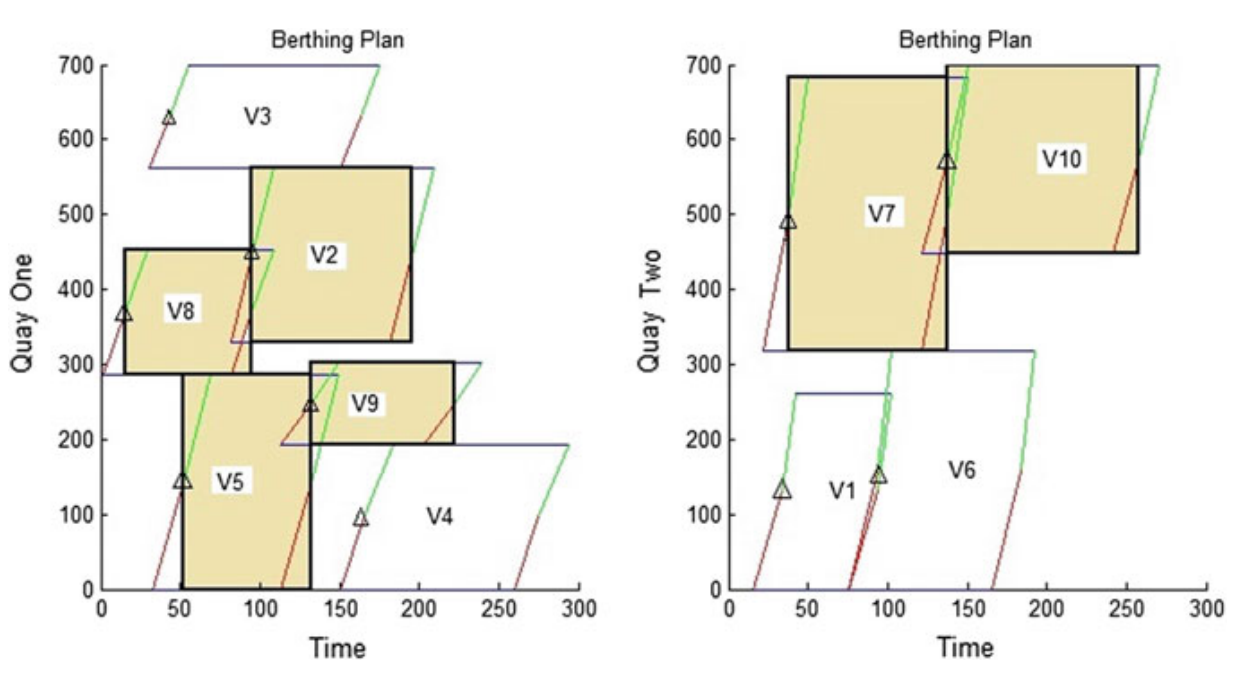
\includegraphics[width=0.7\textwidth]{./img/bap-example-fuzzy-solution.png}
\caption{\label{fig:bap-example-solution}Example solution of a fuzzy BAP model over multiple quays. The parallelograms represent the fuzzy solution visually by depicting the lower and upper bounds for the arrival and departure times with the vertial sloped lines. The yellow filled squares represent the average crisp solution.}
\end{figure}

\section{Summary}
\label{sec:org046f717}
In this section the state of the art for BEB charging was discussed. The various problems of interest and solution
methods for charging BEBs were outlined. Specifically this included: BEB assignment, infrastructure optimization,
charge modeling, robust modeling, and the BAP/PAP model. The problem description for the proposed work was then provided
along with a short introduction to MILP, the BAP, and the PAP along with its formulation. An introduction to fuzzy set
theory was provided followed by a description of the FFLP. A model for the Fuzzy BAP was then discussed along with an
example solution.
\chapter{APPROACH}
\label{sec:approach}
This section introduces the actions and formulations associated with the objectives described in \ref{sec:objectives}. The
actions shall be presented in the same order as \ref{sec:objectives} for consistency. Furthermore, as some of the research
proposed in this work has been completed, this section aims to identify complete and incomplete aspects of the research
as its being presented.

\section{Objective 1: Mathematically model the PAP to optimally assign BEBs to queues with unknown charging times to allow consideration of consumption cost and battery health}
\label{sec:act-math-model-pap}
This section addresses the actions by deriving a method of identifying buses for subsequent visits which is utilized to
formulate a way of estimating the SOC during the BEBs charging phase. The method introduced in this section demonstrates
the linear battery dynamics that have been implemented in the MILP-PAP. The derivation also demonstrates how the model
will discretize the queuing space to accommodate multiple types of chargers.

\subsection{Task 1.1: Modify PAP to enable multiple visits by a BEB with variable charger duration per visit}
\label{sec:app-modify-pap}
Applying the PAP to BEB charging requires four fundamental changes. The first is that the time that a BEB spends
charging is allowed to vary. Thus, \(s_i\) becomes a variable of optimization. Second, in the PAP each charging visit is
assumed to be a different vehicle. For the BEB charging problem, each bus may make multiple visits to the station
throughout the day and the resulting charge for a bus at a given time is dependent upon each of the prior visits made.
The third fundamental change is related to the first two. The charge of each bus must be tracked in the optimization to
ensure that charging across multiple visits is sufficient to allow each bus to execute its route throughout the day. The
final change in the PAP is associated with the fact that the charger is modeled as one continuous bar. For the BEB, it
will be assumed that a discrete number of chargers exist. Moreover, it is assumed that these chargers may have different
charge rates.

The discussion of the four changes are separated into two sections. \autoref{sec:queuing} discusses the changes in the
spatial-temporal constraint formulation to form a queuing constraint. \autoref{sec:batt_dynamics} then discusses the
addition of the bus charge management. This section ends with a brief discussion of a modified objective function and
the statement of the full problem in \autoref{sec:BEB_MILP}. The notation is explained throughout and summarized in
\autoref{tab:variables}.

\subsubsection{Queuing Constraints}
\label{sec:queuing}
\noindent
The queuing constraints ensure that the busses entering the queues for charging are assigned in a feasible manner as
they come into the station. There are three sets to differentiate between different entities. \(\mathbb{B} = \{1, ...,
n_B\}\) is the set of bus indices with index \(b\) used to denote an individual bus, \(\mathbb{Q} = \{1, ..., n_Q\}\) is the set of
queues with index \(q\) used to denote an individual queue, and \(\mathbb{V} = \{1, ..., n_V\}\) is a set of visits to the
station with \(i,j\) used to refer to individual visits. The mapping \(\Gamma: \mathbb{V} \rightarrow \mathbb{B}\) is used to map a visit
index to a bus index with the shorthand \(\Gamma_i\) used to refer to the bus index for visit \(i\).

Most variables are now defined in terms of a visit. Two separate visits could correspond to different buses or visits by
the same bus. The PAP spatial variable, \(s_i\), is removed and \(v_i\) is made to be an integer corresponding to which
queue visit \(i\) will be using. Thus, when \(\psi_{ij} = 1\), vehicle \(i\) is queued to a charger that has a larger index than
the charger that vehicle \(j\) is queued, i.e., \(v_i-v_j \geq 1\). The variable \(S\) is likewise replaced with \(n_Q\). Note that
\(n_Q = n_B + n_C\), where \(n_B\) is the number of busses and \(n_C\) is the number of chargers. The rationale for having
more queues than chargers is to allow buses to sit idle instead of requiring the bus to charge at each visit. The
modified queuing constraints can be written as shown in \autoref{eq:packconstrs}.

\begin{subequations}
\label{eq:packconstrs}
\begin{align}
    v_i - v_j - (\psi_{ij} - 1)n_Q \geq 1       \label{subeq:space}        \\
    d_i \leq \tau_i                             \label{subeq:valid_depart} \\
    s_i \geq 0                               \label{subeq:pos_charge} \\
    v_i \in \mathbb{Q}                       \label{subeq:vspace}
\end{align}
\end{subequations}

The constraint in \autoref{subeq:space} is nearly identical to \autoref{subeq:bapspace}, but rather than viewing the
charger as a continuous strip of length \(S\), it is discretized into \(n_Q\) queues a width of unit length one. A BEB is
also assigned a unit length of one which is reflected in \autoref{subeq:space} by \(\cdot \geq 1\). \autoref{subeq:valid_depart}
ensures that the time the BEB is detatched from the charger, \(d_i\), is before its departure time, \(\tau_i\).
\autoref{subeq:vspace} defines the integer set of indices for queues for \(v_i\).

\subsubsection{Battery Charge Dynamic Constraints}
\label{sec:batt_dynamics}
Battery dynamic constraints are now introduced to relate busses to visits and guarantee that buses have sufficient time
to charge. Two constraints are enforced on the bus charge: busses must always have sufficient charge to execute their
respective routes and each bus must end the day with a specific charge threshold, preparatory for the next day.

The charge at the beginning of visit \(i\) is denoted as \(\eta_i\). As a charge on the bus is dependent upon the visits that
bus makes to the station, the mapping \(\Upsilon: \mathbb{V} \rightarrow \mathbb{V} \bigcup \{\varnothing\}\) is used to determine the next visit
that corresponds to the same bus, with \(\Upsilon_i\) being shorthand notation. Thus, \(\Gamma_j\) and \(\Gamma_{\Upsilon_i}\), for \(\Upsilon_i = j\), would
both map to the same bus index as long as \(\Upsilon_i\) is not the null element, \(\varnothing\). That is, \(\Gamma_{\Upsilon_i}\) where \(\Upsilon_i =
0\) indicates that there are no future visits for bus \(i\).

To drive time spent on the charger, \(s_i\), as well as define initial, final, and intermediate bus charges for each visit
\(i\), the sets for initial and final visits must be defined. Let the mapping of the first visit by each bus be denoted as
\(\Gamma^0_i : \mathbb{B} \rightarrow \mathbb{V}\). The indexed value of \(\Gamma^0_i\) represents the index for the first visit of bus \(b\) or
the null element, \(\varnothing\). Similarly, let \(\Gamma^f_i : \mathbb{B} \rightarrow \mathbb{B}\) contain the indexes for the final
visit of each bus \(b\) or the null element. The initial and final bus charge percentages, \(\alpha\) and \(\beta\), can then be
represented by the constraint equations \(\eta_{\Gamma^0_i} = \alpha \kappa_{\Gamma^0_i}\) and \(\eta_{\Gamma^f_i} = \beta \kappa_{\Gamma^f_i}\), respectively. The
intermediate charges must be determined at solve time.

It is assumed that the charge received is proportional to the time spent charging. The charge rate for charger \(q\) is
denoted as \(r_q\). Note that a value of \(r_q = 0\) corresponds to a queue where no charging occurs. A bus in such a queue
is simply waiting for the departure time. The queue indices are ordered such that the final \(n_B\) queues have \(r_q = 0\)
to allow an arbitrary number of buses to sit idle at any given moment in time. The amount of discharge between visits
\(i\) and \(\Upsilon_i\), the next visit of the same bus, is denoted as \(\Delta_i\). If visit \(i\) occurred at charger \(q\), the charge of
the bus coming into visit \(\Upsilon_i\) would be \(\eta_{\Upsilon_i} = \eta_i + s_i r_q - \Delta_i\).

The binary decision variable \(w_{iq}\) is introduced to determine whether visit \(i\) uses charger \(q\). This allows the
charge of the bus coming into visit \(\Upsilon_i\) to be written in summation form as

\begin{subequations}
    \label{subeq:pre_next_charge}
\begin{align}
    \eta_{\Upsilon_i} = \eta_i + \sum_{q=1}^{n_Q} s_i w_{iq} r_q - \Delta_i  \\
    \sum_{q=1}^{n_Q} w_{iq} = 1 \\
    w_{iq} \in \{0,1\}
\end{align}
\end{subequations}

The choice of queue for visit \(i\), becomes a slack variable and is defined in terms of \(w_{iq}\) as

\begin{equation}
    v_i = \sum_{q=1}^{n_Q} qw_{iq}
\end{equation}

Maximum and minimum values for the charges are included to ensure that the battery is not overcharged and to guarantee
sufficient charge for subsequent visits. The upper and lower battery charge bounds for bus \(b\) are \(\kappa_b\) and \(\nu_b \kappa_b\),
respectively0 \(\kappa_b\) is the battery capacity and \(\nu_b\) is a percent value. As \(\eta_i\) corresponds to the charge at the
beginning of the visit, the upper bound constraint must also include the charge received during the visit as follows.

\begin{subequations}
    \label{subeq:pre_min_max}
\begin{align}
    \eta_i + \sum_{q=1}^{n_Q} s_i w_{iq} r_q \leq \kappa_{\Gamma_i}                 \\
    \eta_i \geq \nu_{\Gamma_i} \kappa_{\Gamma_i}
\end{align}
\end{subequations}

Note that the term \(s_i w_{iq}\) is a bilinear term. A standard way of linearizing a bilinear term that contains an
integer variable is by introducing a slack variable with an either/or constraint
\cite{chen-2010-applied,rodriguez-2013-compar-asses}. Allowing the slack variable \(g_{iq}\) to be equal to \(s_i w_{iq}\),
\(g_{iq}\) can be defined as

\begin{equation}
    \label{eq:giq_cases}
    g_{iq} =
    \begin{cases}
        s_i & w_{iq} = 1 \\
        0 & w_{iq} = 0
    \end{cases}.
\end{equation}

\autoref{eq:giq_cases} can be expressed as a mixed integer constraint using big-M notation with the following four
constraints.

\begin{subequations}
    \label{eq:slack_gain}
\begin{align}
    s_i - (1 - w_{iq})M \leq g_{iq}  \label{subeq:repgpgret} \\
    s_i \geq g_{iq}                 \label{subeq:repgples} \\
    Mw_{iq} \geq g_{iq}              \label{subeq:repgwgret} \\
    0 \leq g_{iq}                   \label{subeq:repgwles}
\end{align}
\end{subequations}

\noindent
where \(M\) is a large value. If \(w_{iq} = 1\) then \autoref{subeq:repgpgret} and \autoref{subeq:repgples} become \(s_i \leq
g_{iq}\) and \(s_i \geq g_{iq}\), forcing \(s_i = g_{iq}\) with \autoref{subeq:repgwgret} being inactive. If \(w_{iq} = 0\),
\autoref{subeq:repgpgret} is inactive and \autoref{subeq:repgwgret} and \autoref{subeq:repgwles} force \(g_{iq} = 0\).

\subsubsection{The BEB Charging Problem}
\label{sec:BEB_MILP}
The goal of the MILP is to utilize chargers as little as possible to reduce energy costs with the fast charging being
penalized more to reduce battery damage. Thus, an assignment cost \(m_q\) and usage cost \(\epsilon_q\) are associated with each
charger, \(q\). These weights can be adjusted based on charger type or time of day that the visit occurs. The assignment
term takes the form \(w_{iq}m_q\), and the usage term takes the form \(g_{iq} \epsilon_q\). The resulting BEB charging problem is
defined in \autoref{eq:objective}.

\begin{equation}
\label{eq:objective}
	\min \sum_{i=1}^N \sum_{q=1}^{n_Q} \Big( w_{iq} m_q + g_{iq} \epsilon_q \Big) \\
\end{equation}

Subject to the constraints

\begin{multicols}{2}
\begin{subequations}
                                                     \label{eq:dynconstrs}
\begin{equation}
    u_i - u_j - s_j - (\sigma_{ij} - 1)T \geq 0              \label{subeq:m_time}         \\
\end{equation}
\begin{equation}
    v_i - v_j - (\psi_{ij} - 1)n_Q \geq 1                  \label{subeq:m_space}        \\
\end{equation}
\begin{equation}
    \sigma_{ij} + \sigma_{ji} + \psi_{ij} + \psi_{ji} \geq 1            \label{subeq:m_valid_pos}    \\
\end{equation}
\begin{equation}
    \sigma_{ij} + \sigma_{ji} \leq 1                              \label{subeq:m_sigma}        \\
\end{equation}
\begin{equation}
    \psi_{ij} + \psi_{ji} \leq 1                              \label{subeq:m_delta}        \\
\end{equation}
\begin{equation}
    s_i + u_i = d_i                                  \label{subeq:m_detach}       \\
\end{equation}
\begin{equation}
    \eta_{\Gamma^0_i} = \alpha \kappa_{\Gamma^0_i}                           \label{subeq:init_charge}    \\
\end{equation}
\begin{equation}
    a_i \leq u_i \leq (T - s_i)                            \label{subeq:m_valid_starts} \\
\end{equation}
\begin{equation}
    d_i \leq \tau_i                                        \label{subeq:m_valid_depart} \\
\end{equation}
\begin{equation}
    \eta_i + \sum_{q=1}^{n_Q} g_{iq} r_q - \Delta_i = \eta_{\gamma_i}   \label{subeq:next_charge}    \\
\end{equation}
\begin{equation}
    \eta_i + \sum_{q=1}^{n_Q} g_{iq} r_q - \Delta_i \geq \nu \kappa_{\Gamma_i} \label{subeq:min_charge}     \\
\end{equation}
\begin{equation}
    \eta_i + \sum_{q=1}^{n_Q} g_{iq} r_q \leq \kappa_{\Gamma_i}         \label{subeq:max_charge}     \\
\end{equation}
\begin{equation}
    \eta_{\Gamma^f_i} \geq \beta \kappa_{\Gamma^f_i}                          \label{subeq:final_charge}   \\
\end{equation}
\begin{equation}
    s_i - (1 - w_{iq})M \leq g_{iq}                     \label{subeq:gpgret}         \\
\end{equation}
\begin{equation}
    s_i \geq g_{iq}                                     \label{subeq:gples}          \\
\end{equation}
\begin{equation}
    Mw_{iq} \geq g_{iq}                                 \label{subeq:gwgret}         \\
\end{equation}
\begin{equation}
    0 \leq g_{iq}                                       \label{subeq:gwles}          \\
\end{equation}
\begin{equation}
    v_i = \sum_{q=1}^{n_Q} qw_{iq}                      \label{subeq:wmax}           \\
\end{equation}
\begin{equation}
    \sum_{q=1}^{n_Q} w_{iq} = 1                         \label{subeq:wone}           \\
\end{equation}
\begin{equation}
   w_{iq}, \sigma_{ij}, \psi_{ij} \in \{0,1\}\;            \label{subeq:binaryspace}        \\
\end{equation}
\begin{equation}
    v_i, q_i \in  \mathbb{Q}                                         \label{subeq:Qspace}        \\
\end{equation}
\begin{equation}
    i \in \mathbb{V}                                   \label{subeq:Ispace}         \\
\end{equation}
\end{subequations}
\end{multicols}

\autoref{subeq:m_time}-\autoref{subeq:m_valid_depart} are reiterations of the queuing constraints in
\autoref{eq:packconstrs}. \autoref{subeq:init_charge}-\autoref{subeq:final_charge} provide the battery charge
constraints. \autoref{subeq:gpgret} through \autoref{subeq:gwles} define the charge gain of every visit/queue
pairing. The last constraints \autoref{subeq:binaryspace}-\autoref{subeq:Ispace} define the sets of valid values for each
variable.

\subsection{Task 1.2: Incorporate heterogeneous charger capabilities into the PAP to model slow and fast charging, and minimize total charger count. Slow charging will be incentivized for battery health and consumption cost.}
\label{sec:app-incorporate-pap}
The kernel of this task was developed in \ref{sec:queuing}; however, some refinement on the formulation of some of the
decision variables is required. To encourage the MILP PAP problem to utilize the fewest number of chargers, the value of
\(m_q\) in the objective function, \ref{eq:objective}, is to be defined as \(\forall q \in \{0, 1, ..., n_B\}: m_q = 0\) and \(\forall q \in
\{n_B+1, n_B+2, ..., n_B + n_C\}: m_q = 1000q\). That is, for each charging queue beyond the idle queues, \(n_B\), increase
the cost of assignment by 1000. By minimizing the objective function, the result will tend toward the fewest number of
charging queues. Furthermore, if we allow the queue to be arranged with slow chargers first and fast chargers second,
then objective function will in addition favor slow chargers.

To account for the consumption cost, consider the charge duration scalar, \(\epsilon_q\). If the input parameter is defined as
the charge rate, \(\epsilon_q = r_q\), then the second term in \ref{eq:objective} defines the consumption cost over visit \(i\),
\(g_{iq}\epsilon_q\). By summing over all visits, the total consumption cost is determined. This metric is thus utilized as a
measure of the consumption cost as well as a mechanism to encourage the model to minimize active charger times,
particuarly for the fast chargers.

\section{Objective 2: Develop robust charger allocation capabilities to account for BEB arrival time uncertainties and non-linear battery dynamics}
\label{sec:act-math-model-robust}
In this section, non-linear dynamics will be introduced with a brief description of the mathematical approach that
will be taken. Proceeding this, the Fuzzy PAP (FPAP) shall be introduced in its entirety. The work presented in this
section has yet to be completed.

\subsection{Task 2.1: Incorporate non-linear battery dynamics into the FFLP PAP model}
\label{sec:non-linear-battery-dynamics}
Modeling the charging dynamics is imperative to the model's accuracy as it is one of the main factors in terms of the
decision variables. If the SOC is improperly modeled, that will produce an erroneous depiction of the state of BEB
charges and could result in over or under charging. Thus, care must be taken into considering the BEB's charging model.
There are various methods of modeling the SOC of a battery and can vary in complexity based on the attempt to
incorporate temperature, battery degradation, and current
\cite{zhang-2021-optim-elect,chen-2008-desig-grey,watrin-2012-multip-lithium}.

Some of the conventional methods to charge batteries are: Constant Voltage (CV), Constant Current (CC), and Constant
Current Constant Voltage (CCCV) \cite{arabsalmanabadi-2018-charg-techn}. CCCV, as the name describes, is the
combination of CCCV model \cite{abdollahi-2016-optim-batter,chen-2008-desig-grey,wang-2021-resear-optim}. In CCCV,
a constant current is applied to a battery until it reaches terminal voltage. At this point a constant voltage is
applied as the charge current decreases and the battery reaches full charge \cite{chen-2008-desig-grey}. Thus, by
extension, CV merely applies a constant voltage and CC a constant current.

As previously stated, the SOC can be accurately modeled until the battery reaches a charge of about 80\%
\cite{liu-2020-batter-elect}. At this point the SOC becomes non-linear. Naturally, it has been suggested by
\cite{zhang-2021-optim-elect} that the SOC can be broken down into a linear and non-linear component. A plot of the SOC
for a battery is shown in \ref{fig:soc-plot} to demonstrate these components \cite{zhang-2021-optim-elect}.

\begin{figure}[htbp]
\centering
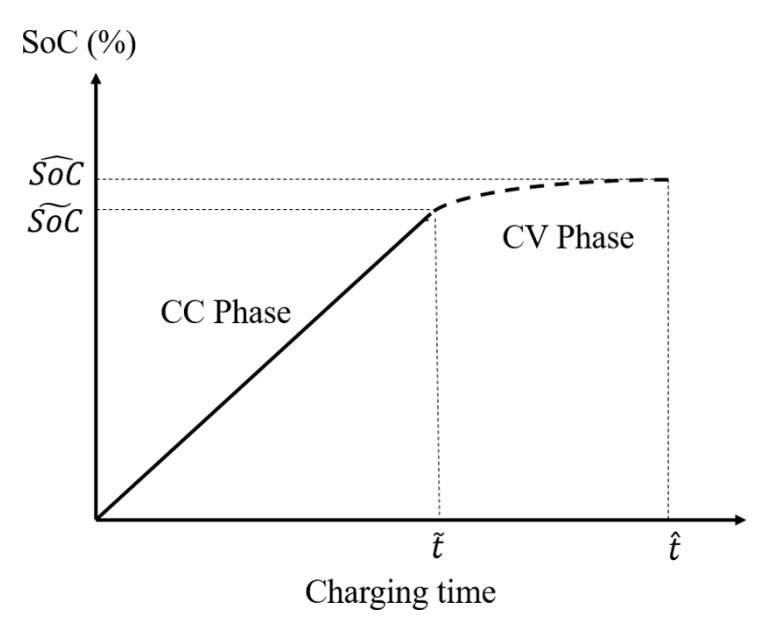
\includegraphics[width=0.5\textwidth]{img/soc-plot.png}
\caption{\label{fig:soc-plot}Illistration of non-linear charging profile.}
\end{figure}

While some leverage the linear and non-linear components to derive their SOC model \cite{abdollahi-2016-optim-batter},
others have derived a first order equation to model this behavior \cite{whitaker-2023-a-network}. Assume that a charge
will occur over \(dt\) seconds. The SOC on the time step \(h+1\) for bus \(i\) can be determined by the simple discrete first
order equation

\begin{equation}
  \eta_{\xi_i} = \bar{a}_q \eta_i - \bar{b}_q \kappa_{\Xi_i}
\end{equation}

where

\begin{equation}
\begin{array}{cc}
  \bar{a}_q = e^{a_q dt} & \bar{b}_q = e^{a_q dt} - 1
\end{array}
\end{equation}

The equation is developed by using exact discretization \cite{hespanha-2018-linear}, and is proved in
\cite{whitaker-2023-a-network}. In the same way as the linear dynamics, the \(i^{\text{th}}\) visit's initial charge is
indicated by \(\eta_i\), the identity of visit \(i\) is \(\eta_{\Xi_i}\), and the subsequent visit is indicated by \(\eta_{\xi_i}\). Thus,
the propagation mechanics remain untouched while the underlying battery dynamics are more accurate.

\subsection{Task 2.2: Model the PAP as an FFLP to allow for uncertain BEB arrival/charge/departure times. An optimal solution shall be produced, but with added flexibility to its application.}
\label{sec:the-fuzzy-pap}
This section derives the Fuzzy PAP (FPAP). It is separated into three parts to construct each component individually:
objective function, queuing constraints, and charging constraints. Before deriving the FPAP, it is prudent to define the
set of fuzzy variables. Similarly to the Fuzzy BAP, the arrival times, \(\tilde{a}_i\), berthing time \(\tilde{u}_i\), and
detach time from the charger \(\tilde{d}_i\) are assumed to be imprecise. Thus, indirectly, the service time,
\(\tilde{s}_i\), the linearization constraint in \ref{eq:slack_gain}, \(\tilde{g}_{iq}\), and the initial charge for visit
\(i\), \(\tilde{\eta}_i\) will also become fuzzy values. Note for the sake space, constraints and objective functions shall be
written in their fuzzy form; however, in practice the equations will be expanded as described in
\ref{sec:fuzzy-preliminaries}.

\subsubsection{Objective Function}
\label{sec:org40dbe71}
Begin by rewriting the crisp objective function with the fuzzy linearization term as shown in \ref{eq:fuzzy-objective}.

\begin{equation}
\label{eq:fuzzy-objective}
\text{min } \sum_{i=1}^{n_I} \sum_{q=1}^{n_Q} \Big( w_{iq} m_q + \tilde{g}_{iq} \epsilon_{q} \Big)
\end{equation}

As shown in \ref{sec:fully-fuzzy-linear-programming}, the method of handling the fuzzy values in the objective function is to
simply apply a ranking function. Let \(\mathfrak{R}\) be defined as the First Index of Yager as shown in \ref{eq:first-index-yager}.
The resulting objective function is shown in \ref{eq:fuzzy-objective-yager}.

\begin{equation}
\label{eq:fuzzy-objective-yager}
\text{min } \sum_{i=1}^{n_I} \sum_{q=1}^{n_Q} \Big( w_{iq} m_q + \mathfrak{R}(g_{iq}) \epsilon_{q} \Big)
\end{equation}

\subsubsection{Queuing Constraints}
\label{sec:org61f75ed}
To derive the queuing constraints, the set of crisp constraints that are of interest are rewritten in terms of the fuzzy
variables that have been identified prior as shown in \ref{eq:fuzzy-packing-constrs}. \ref{subeq:fp_m_time} fuzzifies all the
temporal terms. \ref{subeq:fp_m_valid_pos} and \ref{subeq:fp_m_sigma} duplicate the constraints \(|\tilde{u}_i|\) times.
Using triangular fuzzy numbers, that would imply constraints for the lower, middle, and upper bounds of the temporal
impreciseness. Similarly, \ref{subeq:fp_m_detach}-\ref{subeq:fp_m_valid_depart} are equivalent to their crisp
counterparts, but with fuzzified terms. \ref{subeq:fp_binaryspace} simply updates the binary decision term.

\begin{multicols}{2}
\begin{subequations} \label{eq:fuzzy-packing-constrs}
\begin{equation}
    \tilde{u}_i - \tilde{u}_j - \tilde{s}_j - (\sigma_{ij} - 1)T \geq 0 \label{subeq:fp_m_time}         \\
\end{equation}
\begin{equation}
    \sigma_{ij} + \sigma_{ji} + \psi_{ij} + \psi_{ji} \geq 1                     \label{subeq:fp_m_valid_pos}    \\
\end{equation}
\begin{equation}
    \sigma_{ij} + \sigma_{ji} \leq 1                                       \label{subeq:fp_m_sigma}        \\
\end{equation}
\begin{equation}
    \tilde{s}_i + \tilde{u}_i = \tilde{d}_i                       \label{subeq:fp_m_detach}       \\
\end{equation}
\begin{equation}
    \tilde{a}_i \leq \tilde{u}_i \leq (T - \tilde{s}_i)                 \label{subeq:fp_m_valid_starts} \\
\end{equation}
\begin{equation}
    \tilde{d}_i \leq \tau_i                                             \label{subeq:fp_m_valid_depart} \\
\end{equation}
\begin{equation}
   \sigma_{ij}, \psi_{ij} \in \{0,1\}\;                                   \label{subeq:fp_binaryspace}        \\
\end{equation}
\end{subequations}
\end{multicols}

\subsubsection{Charging Constraints}
\label{sec:orga5b2265}
Similarly to the other derivations, the crisp constraints are rewritten with their equivalent fuzzy terms.
\ref{subeq:fp_init_charge}-\ref{subeq:fp_final_charge} are equivalent to their crisp counterpart with the added lower
and upper bounds for the battery charge for visit \(i\). Note that the discharge amount, \(\Delta_i\), is not fuzzy. It is
assumed that the bus traveled the same distance during the route, thus the same amount of discharge. This is done as a
simplification to the estimation of the discharge of a BEB over its given route.
\ref{subeq:fp_gpgret}-\ref{subeq:fp_gwles} fuzzify the linearization terms in a similar manner, but the crisp spatial
term, \(w_{iq}\) is included. The inclusion of the crisp terms with the fuzzy values are allowed because although the time
may be allowed to fluctuate, the specified queue, discharge amounts, or initial/final charge times are the same for each
element of the fuzzy temporal values. Thus, when the fuzzy constraints are converted into crisp constraints, the
constraint validity is maintained \cite{ghanbari-2019-fuzzy}.

\begin{multicols}{2}
\begin{subequations}                                                       \label{eq:fuzzy-dyn-constrs}
\begin{equation}
    \tilde{\eta}_{\Gamma^0_i} = \alpha \kappa_{\Gamma^0_i}                                        \label{subeq:fp_init_charge}    \\
\end{equation}
\begin{equation}
    \tilde{\eta}_i + \sum_{q=1}^{n_Q} \tilde{g}_{iq} r_q - \Delta_i = \tilde{\eta}_{\gamma_i} \label{subeq:fp_next_charge}    \\
\end{equation}
\begin{equation}
    \tilde{\eta}_i + \sum_{q=1}^{n_Q} \tilde{g}_{iq} r_q - \Delta_i \geq \nu \kappa_{\Gamma_i}       \label{subeq:fp_min_charge}     \\
\end{equation}
\begin{equation}
    \tilde{\eta}_i + \sum_{q=1}^{n_Q} \tilde{g}_{iq} r_q \leq \kappa_{\Gamma_i}               \label{subeq:fp_max_charge}     \\
\end{equation}
\begin{equation}
    \tilde{\eta}_{\Gamma^f_i} \geq \beta \kappa_{\Gamma^f_i}                                        \label{subeq:fp_final_charge}   \\
\end{equation}
\begin{equation}
    \tilde{s}_i - (1 - w_{iq})M \leq \tilde{g}_{iq}                           \label{subeq:fp_gpgret}         \\
\end{equation}
\begin{equation}
    \tilde{s}_i \geq \tilde{g}_{iq}                                           \label{subeq:fp_gples}          \\
\end{equation}
\begin{equation}
    Mw_{iq} \geq \tilde{g}_{iq}                                               \label{subeq:fp_gwgret}         \\
\end{equation}
\begin{equation}
    0 \leq \tilde{g}_{iq}                                                     \label{subeq:fp_gwles}          \\
\end{equation}
\end{subequations}
\end{multicols}

\section{Project Schedule}
\label{sec:org5711130}
The following Gantt chart, shown in \autoref{fig:gantt}, plots out the work that has been completed and the work to be
completed. The estimated completion date is mid to late-November. Note that the blocks before the \texttt{TODAY} mark in
\autoref{fig:gantt} is work that has been previously completed or is work in progress.

\begin{figure}[ht]
  \begin{ganttchart}[
    vgrid={*{11}{gray, dotted}, *1{black, dashed}},
    bar label node/.append style={
      align=left,
      text width=width("Aim 2. Software verificationx")},
    today=21
    ]{1}{24}
    \gantttitle{2022}{12} \gantttitle{2023}{12} \\
    \gantttitlelist{1,...,24}{1} \\
    \ganttbar{MILP-PAP}{1}{12} \\
    \ganttbar{SA-PAP}{9}{21} \\
    \ganttbar{Non-Linear Battery Dynamics}{20}{21} \\
    \ganttbar{Fuzzy PAP}{18}{23} \\
    \ganttbar{Defense}{23}{24} \\
  \end{ganttchart}
  \caption{Gantt chart for the proposed work.}
  \label{fig:gantt}
\end{figure}

\section{Summary}
\label{sec:approach-summary}
The previous sections discussed the approaches to be taken (or have taken) for each respective objective along with a
derivation when available for the proposed approach. A projected project schedule was also provided. This research
intends to increase utility of the PAP by first modifying the model to allow BEBs' charges to be propagated, include an
identifier for BEBs to be tracked, utilize non-linear charging dynamics, as well as utilizing FFLP to develop a robust
solution. Upon completion, the proposed research will demonstrate its full utility and extensibility due to the MILP's
nature of adding additional constraints. This research project shall illustrate a robust BEB charging schedule with
realistic applicability.

\references{citation-database/lib-ref,citation-database/lit-ref}{IEEEtran}
\end{document}
